% ______________________________________________________________________________
%
% DVG001 -- Introduktion till Linux och små nätverk
%                                     Projektarbete
% ~~~~~~~~~~~~~~~~~~~~~~~~~~~~~~~~~~~~~~~~~~~~~~~~~
% Author:   Jonas Sjöberg
%           tel12jsg@student.hig.se
%
% Date:     2016-06-07 -- 2016-06-13
%
% License:  Creative Commons Attribution 4.0 International (CC BY 4.0)
%           <http://creativecommons.org/licenses/by/4.0/legalcode>
%           See LICENSE.md for additional licensing information.
% ______________________________________________________________________________


\section{Skapande av IPv6-tunnel}
% ______________________________________________________________________________
\subsection{Registrering av tunnelservice}
För tunnel-service valdes gratistjänsten ``Tunnel Broker''
\cite{ipv6:tunnelbroker} som erbjuds av Hurricane Electric.  
Som ett första steg registrerades ett nytt konto. Sedan skapades en tunnel
genom Hurricane Electrics web-interface för inloggade användare. 
Detta visas i Figur~\ref{fig:01}.

\screenshot{include/01_tunnelbroker_new-tunnel}
           {Skärmdump på skapande av en ny tunnel.}
           {Skärmdump på skapande av en ny IPv6-tunnel i Hurricane Electrics
            web-interface.}
           {fig:01}


\subsection{Statisk IP-adress för Debian-maskinen}
För att ge Debian-maskinen en statisk IP-adress ändrades filen
\texttt{/etc/network/interfaces} för att få utseendet enligt
Programlistning~\ref{listing:interfaces-static-ip}.

\configsource{include/conf_interfaces-static-ip}
            {Innehåll i konfigurationsfilen \texttt{/etc/network/interfaces}
 					   för statisk IP-adress.}
            {listing:interfaces-static-ip}


\subsection{Konfiguration av router}
I nätverkets routern reserveras en IP-adressen \texttt{192.168.1.112} till
Debian-maskinens MAC-adress.


\subsection{Konfiguration av tunneln}
Konfigurationen av tunneln sköts också genom att ändra i filen
\texttt{/etc/network/interfaces}, som får utseendet enligt
Programlistning~\ref{listing:interfaces-all}.

\configsource{include/conf_interfaces-all}
						 {Fullständigt innehåll i konfigurationsfilen
							\texttt{/etc/network/interfaces}.}
             {listing:interfaces-all}


Raden \texttt{auto heipv6} gör att tunneln startas automatiskt.
Efter omstart visas den nya tunneln bland aktiva interface. Detta visas i  
Programlistning~\ref{listing:ifconfig}.

\shellsource{include/cmd_ifconfig}
            {Verifiering av ändringar i \texttt{/etc/network/interfaces}
             genom körning av \texttt{ifconfig}.}
            {listing:ifconfig}

Brandväggen \texttt{ufw} ställs in att tillåta all trafik från Hurricane
Electrics IP-adress \texttt{216.66.80.90} genom att köra kommandot \texttt{sudo
ufw allow proto ipv6 from 216.66.80.90}.

% ______________________________________________________________________________
\subsection{Test av tunneln}
Anslutningen testas genom att köra kommandon enligt 
Programlistning~\ref{listing:ip_addr-route} och \ref{listing:ping6}.

\shellsource{include/cmd_ip_addr-route}
            {Kontroll av IPv6-tunnelns status.}
            {listing:ip_addr-route}

\shellsource{include/cmd_ping6}
            {Test av ICMP/ping till server över IPv6.}
            {listing:ping6}

Anslutningen verifieras också med hemsidorna \texttt{http://test-ipv6.com/} och
\texttt{http://ipv6-test.com/} enligt skärmdumpar i Figur~\ref{fig:02} och
Figur~\ref{fig:03}.
Anslutning till servern \texttt{http://rigel.hig.se} visas i
Figur~\ref{fig:04}.

\screenshot{include/02_ipv6test}
           {Skärmdump på test av anslutningar.}
					 {Skärmdump på test av anslutningar till nätverket med tjänsten
						\texttt{http://ipv6-test.com/}.}
           {fig:02}

\screenshot{include/03_test-ipv6}
           {Skärmdump på test av anslutningar.}
           {Skärmdump på test av anslutningar till nätverket med tjänsten
            \texttt{http://test-ipv6.com/}.}
           {fig:03}

\screenshot{include/04_rigel-hig-se}
           {Skärmdump på test av anslutning.}
					 {Skärmdump på test av IPv6 genom anslutning till
						\texttt{http://rigel.hig.se}.}
           {fig:04}


% ______________________________________________________________________________
\subsection{Nätverksmodell}
Nätverkets konfiguration illustreras i Figur~\ref{fig:networkgraph}.

\begin{figure}[H]
  \centering
  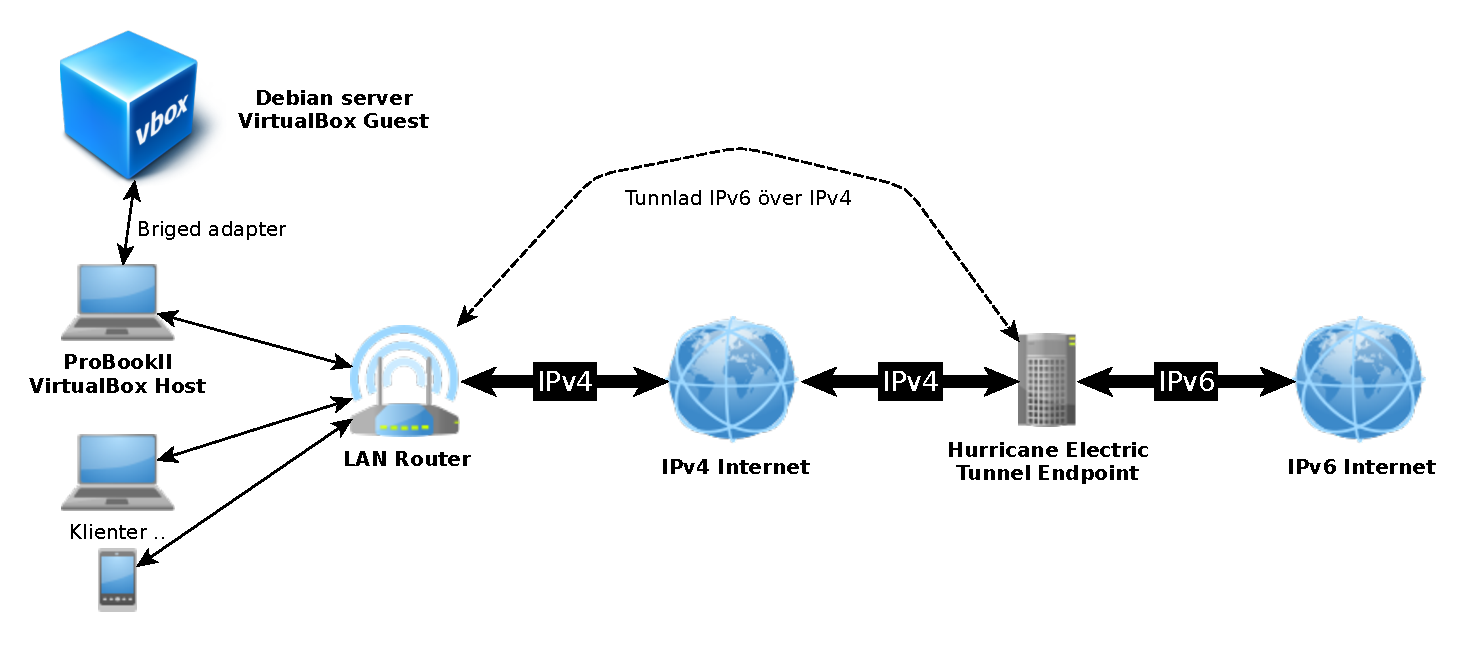
\includegraphics[width=\linewidth]{include/networkgraph}
  \caption[Diagram över nätverkets konfiguration.]
          {Övergripande konceptuellt diagram över nätverkets
           konfiguration.}
  \label{fig:networkgraph}
\end{figure}

I modellen visas Debian-servern som är en VirtualBox virtuell maskin, till
vänster. Debian-serverns nätverkstyp är inställd till \texttt{Bridged}, vilket
innebär att värdmaskinen filtrerar ut trafik som är ämnad gästsystemet, på så
vis att gästsystemet verkar vara kopplat direkt till värdsystemets
nätverksadapter.
